\documentclass[tikz,border=3mm,multi=tikzpicture]{standalone}
\usepackage[utf8]{inputenc}
\usepackage[T1]{fontenc}
\usepackage{helvet}
\renewcommand{\familydefault}{\sfdefault}
\usepackage{tikz}
\usetikzlibrary{angles,quotes,calc,intersections}
\begin{document}

\tikzset{every node/.append style={font=\sffamily\small}}
% TikZ 1
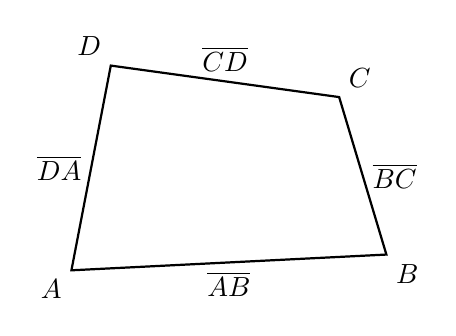
\begin{tikzpicture}[scale=1]
\coordinate (A) at (0,0); \coordinate (B) at (4,0.2); \coordinate (C) at (3.4,2.2); \coordinate (D) at (.5,2.6);
\draw[thick] (A)--(B)--(C)--(D)--cycle;
\foreach \p/\pos in {A/below left,B/below right,C/above right,D/above left}{\node[\pos] at (\p) {$\p$};}
\node[below] at ($(A)!0.5!(B)$) {$\overline{AB}$};
\node[right] at ($(B)!0.5!(C)$) {$\overline{BC}$};
\node[above] at ($(C)!0.5!(D)$) {$\overline{CD}$};
\node[left] at ($(D)!0.5!(A)$) {$\overline{DA}$};
\end{tikzpicture}
% TikZ 2
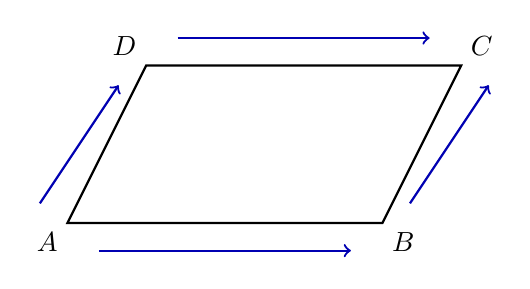
\begin{tikzpicture}[scale=1]
\coordinate (A) at (0,0); \coordinate (B) at (4,0); \coordinate (C) at (5,2); \coordinate (D) at (1,2);
\draw[thick] (A)--(B)--(C)--(D)--cycle;
\draw[blue!70!black,thick,->] (.4,-.35)--(3.6,-.35);
\draw[blue!70!black,thick,->] (1.4,2.35)--(4.6,2.35);
\draw[blue!70!black,thick,->] (-.35,.25)--(.65,1.75);
\draw[blue!70!black,thick,->] (4.35,.25)--(5.35,1.75);
\foreach \p/\pos in {A/below left,B/below right,C/above right,D/above left}{\node[\pos] at (\p) {$\p$};}
\end{tikzpicture}


% TikZ 3
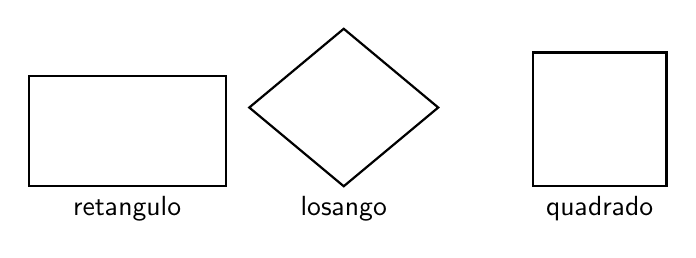
\begin{tikzpicture}[scale=1]
\draw[thick] (0,0) rectangle (2.5,1.4);
\node[below] at (1.25,0) {retangulo};
\draw[thick] (4,0)--(5.2,1)--(4,2)--(2.8,1)--cycle;
\node[below] at (4,0) {losango};
\draw[thick] (6.4,0) rectangle (8.1,1.7);
\node[below] at (7.25,0) {quadrado};
\end{tikzpicture}
% TikZ 4
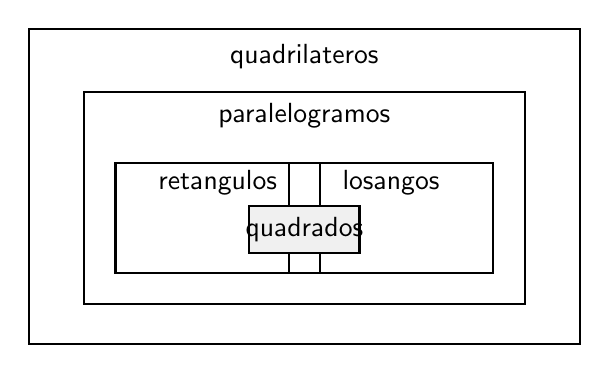
\begin{tikzpicture}[scale=1]
\draw[thick] (0,0) rectangle (7,4);
\node at (3.5,3.65) {quadrilateros};
\draw[thick] (.7,.5) rectangle (6.3,3.2);
\node at (3.5,2.9) {paralelogramos};
\draw[thick] (1.1,.9) rectangle (3.7,2.3);
\node at (2.4,2.05) {retangulos};
\draw[thick] (3.3,.9) rectangle (5.9,2.3);
\node at (4.6,2.05) {losangos};
\draw[thick,fill=gray!12] (2.8,1.15) rectangle (4.2,1.75);
\node at (3.5,1.45) {quadrados};
\end{tikzpicture}


% TikZ 5
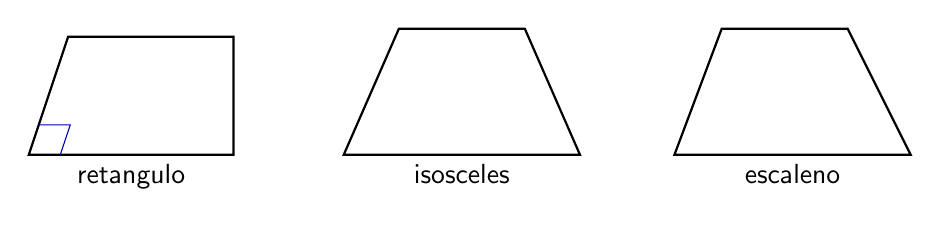
\begin{tikzpicture}[scale=1]
\coordinate (A) at (0,0); \coordinate (B) at (2.6,0); \coordinate (C) at (2.6,1.5); \coordinate (D) at (.5,1.5);
\draw[thick] (A)--(B)--(C)--(D)--cycle;
\pic[draw=blue!70!black, angle radius=4mm] {right angle=D--A--B};
\node[below] at (1.3,0) {retangulo};
\coordinate (E) at (4,0); \coordinate (F) at (7,0); \coordinate (G) at (6.3,1.6); \coordinate (H) at (4.7,1.6);
\draw[thick] (E)--(F)--(G)--(H)--cycle;
\node[below] at (5.5,0) {isosceles};
\coordinate (I) at (8.2,0); \coordinate (J) at (11.2,0); \coordinate (K) at (10.4,1.6); \coordinate (L) at (8.8,1.6);
\draw[thick] (I)--(J)--(K)--(L)--cycle;
\node[below] at (9.7,0) {escaleno};
\end{tikzpicture}
\end{document}
